\documentclass[german,version-2019-11]{uzl-thesis}
\UzLThesisSetup{
  Logo-Dateiname        = {uzl-thesis-logo-itcs.pdf},
  Verfasst              = {am}{Institut für Theoretische Informatik},
  %
  % The titles:
  %
  Titel auf Deutsch     = {
    Algorithmen für bewegende Ziele im Travelling Salesman Problem
  }, 
  Titel auf Englisch    = {
    Algorithms for Moving-Target Travelling Salesman Problem
  },
  Autor                 = {Felix Greuling},
  Betreuerin            = {Prof. Dr. Maciej Liskiewicz},
  Bachelorarbeit,
  Studiengang           = {Informatik},
  Datum                 = {30. Dezember 2019},
  Abstract              = {
    \textcolor{red}{TODO}
    
  },
  Zusammenfassung       = {
    \textcolor{red}{TODO}  
  },
  Acknowledgements      = {

  }, 
  % Alphabetische Bibliographie
  % Alternatively:
  Numerische Bibliographie
}

% \UzLStyle{pagella basic design}
% \UzLStyle{pagella centered design}
% \UzLStyle{pagella contrast design}
% \UzLStyle{alegrya basic design}
% \UzLStyle{alegrya scholary design}
% \UzLStyle{alegrya stylish design}
\UzLStyle{alegrya modern design}
% \UzLStyle{thesis black and white structure}

% Now, include the package you need here using \usepackage. 
% \usepackage{graphicx,float,wrapfig}
\usepackage{mathtools}
\usepackage{algorithm}
\usepackage{algpseudocode}

%tikz
\tikzstyle{gray}  = [thick, color=gray, circle, draw]
\tikzstyle{red}   = [thick, color=red, circle, draw]
\tikzstyle{blue}  = [thick, color=blue, circle, draw]
\tikzstyle{green} = [thick, color=green, circle, draw]

% begin of the document
\begin{document}
% \chapter{Introduction}
\chapter{Einleitung}


%\section{Contributions of this Thesis}
\section{Beiträge dieser Arbeit}



%\section{Related Work}
\section{Verwandte Arbeiten}



%\section{Structure of this Thesis}
\section{Aufbau dieser Arbeit}


\chapter{Grundlagen}
\label{chapter-use}
Im folgenden Kapitel werden alle nötigen Grundlagen für bewegende Ziele im Travelling-Salesman-Problem erläutert. Dabei werden zwei konkrete Fälle vorgestellt:
\begin{enumerate}
\item eindimensionaler Fall: Jedes Ziel kann sich nur auf einer Linie bewegen
\item zwei-orthogonale-Achsen-Fall: Erweitert den eindimensionalen Fall um eine orthogonal, auf der ersten Linie, liegenden Achse, auf der sich die Ziele bewegen können.
\end{enumerate}
Die Approximation für generelle Fälle gilt dabei schwierig, da viele verschiedene Faktoren die Komplexität des Problems bestimmen. Die Approximations-Forschung in \cite{hammar} zeigte, dass sich die Probleme nicht besser als mit einem Faktor von $2^{\pi(\sqrt{\pi})}$, es sei denn $P=NP$. Dies gilt bisher allerdings weiterhin als ungelöstes Problem in der Informatik.

\section{Fallübergreifende Definitionen}
\textcolor{red}{TODO: kleine Einleitung}
\begin{definition} 
\label{def:Ziel}
Jede Instanz enthält eine Anzahl $n$ von Zielen $Z = \{z_1,...,z_n\}$. Jedes Ziel $z_i$ befindet sich zunächst an einem Startpunkt $p_i$ und bewegt sich dann mit einer konstanten Geschwindigkeit $v_i$ entlang einer Achse , $p_i, v_i \in\mathbb{R}$. Die Positionen und Geschwindigkeiten können dabei als Vektoren $P$ und $V$ dargestellt werden.
\begin{align*}
P = (p_1, ..., ,p_n)^T \\
V = (v_1, \; ..., \; ,v_n)^T
\end{align*}
Demnach kann ein Ziel als ein Tupel $z_i = (p_i, v_i)$ dargestellt werden. Der Ursprung ist definiert durch einen Punkt ohne Geschwindigkeit. Das Tupel $(-1,0)$ würde also bedeuten, dass der Verfolger an der Koordinate $-1$ startet und ist durch die Geschwindigkeit von $0$ stationär. Einfachheitshalber wird in dieser Arbeit der Ursprung mit $(0,0)$ für 1D-Fälle fest definiert. Ein Ziel mit einer negativen Koordinate befindet sich auf der linken, positive Koordinaten auf der rechten Seite des Ursprungs. 
\end{definition}

\begin{definition}
Der Verfolger kann sich ebenfalls nur auf den Achsen bewegen. Sein Ziel ist die schnellst mögliche Tour zu finden, um alle Punkte abzufangen. Dabei bewegt sich der Verfolger mit der Maximalgeschwindigkeit 
\begin{align*}
v_{verfolger} > |v_i|, \forall v_i\in V.
\end{align*}

Dies stellt sicher, dass der Verfolger nach einer gewissen Zeit jedes Ziel auf jeden Fall eingeholt hat. Andernfalls würde eine unendlich große Tourzeit berechnet werden. Der Ursprung ist gleichzeitig auch der Ziel der Tour. Demnach startet und endet jede Tour an diesem stationären Punkt.
\end{definition}

\begin{definition}
\label{def:UpdatedPos}
Mit dem Zeitstempel $t\in \mathbb{R}^+_0$ kann genau bestimmt werden, an welcher Position sich ein Ziel hinbewegt hat. Die Position eines Ziels ist also abhängig vom aktuellen Zeitstempel $t$. Jede Tour beginnt bei $t=0$. \\
Es gilt
\begin{align*}
p_{i,t} = p_{i,0} + v_i\cdot t.
\end{align*} 
\end{definition}

\begin{definition}
\label{def:WegZeit}
Die Zeit, die benötigt wird, um ein Ziel $B$ von der Position von Ziel $A$ einzuholen, ist als. 
%v_{verfolger}\cdot\tau + pos_A &= v_{B}\cdot\tau + pos_B \\
%(v_{verfolger}-v_B)\cdot\tau &= pos_B-pos_A \\
\begin{align*}
\tau &= \bigg\vert\frac{\|pos_A,pos_B\|_1}{v_{verfolger}-v_B}\bigg\vert
\end{align*} 
definiert.
Die Berechnung beruht auf der nach der Zeit (in diesem Fall $\tau$) gleichgesetzten und umgestellten physikalischen Formel \footnote{Gleichförmige Bewegung: $s=v\cdot t+s_0$}.
Bemerke, $v_A$ wird durch $v_{verfolger}$ ersetzt, da sich der Verfolger immer mit maximaler Geschwindigkeit bewegt.
\end{definition}

\begin{definition} 
Eine optimale Tour ist die kürzeste Reihenfolge an Zielen, bei dem jedes $z_i\in Z$ eingeholt wurde. Dabei startet und beendet der Verfolger jede Tour im Ursprung. 
\end{definition}

\section{Eindimensionaler Fall}
Der eindimensionale Fall wurde zuerst in \cite{helvig} präsentiert. Die Autoren modellieren das Problem als Graph-Problem, wobei der eigentliche Graph on-the-fly erstellt wird. Mit linearer Programmierung wird anschließend die schnellst mögliche Abfangzeit für jeden Zustand bestimmt. Somit kann die die optimale Tourzeit und -Reihenfolge bestimmt werden.
Im eindimensionalen Fall befinden sich alle Ziele auf einer Achse und können sich nur in zwei verschiedene Richtungen bewegen. Dasselbe gilt auch für den Verfolger. Wichtig ist zunächst die Bedingung, dass der Verfolger sich immer mit seiner maximalen Geschwindigkeit $v_{verfolger}$ bewegt. Helvig et. al. bewiesen dies mit dem Aspekt, dass ein eine Reisegeschwindigkeit von $v<v_{verfolger}$ äquivalent zu einer Wartezeit an einem Punkt ist. Dies resultiert in eine längere Tourzeit, das heißt die Tour wäre nicht mehr optimal.

Um das Problem der kürzesten Route zu lösen, muss sich der Verfolger an einem Ziel entscheiden, das nächste Ziel in derselben oder entgegengesetzte Richtung einzuholen. Die Kostenberechnung für eine schnellste Tour aus
\begin{itemize}
\item alle Ziele links vom Ursprung aus gesehen und danach alle rechten Ziele abfangen
\item alle Ziele rechts vom Ursprung aus gesehen und danach alle linken Ziele abfangen
\end{itemize} 
ist zwar simpel und einfach implementierbar, reicht aber nicht aus (siehe Abbildung \ref{fig:GegenBsp1Dim}).
\begin{figure}[htbp]
\centering
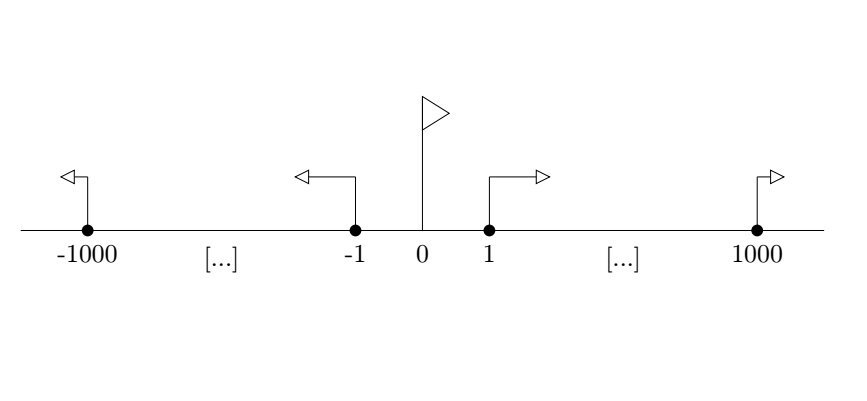
\includegraphics[scale=0.68]{../Grafiken/Verwendete/1DGegenbsp.PNG}
\caption{Offensichtlich würde der Verfolger mit der Geschwindigkeit $v_{verfolger}=11$ deutlich länger für eine Tour brauchen, sofern er zunächst alle Ziele auf der einen und dann auf der anderen Seite abarbeitet. Hierbei wäre es sinnvoll, zunächst die Ziele $(-1,-10)$ und $(1,10)$ einzuholen.}
\label{fig:GegenBsp1Dim}
\end{figure}
Im worst case geht $t\rightarrow\infty$, sobald die äußersten Ziele noch deutlich weiter entfernt vom Ursprung aus liegen. 

Die Autoren aus \cite{helvig} definierten anschließend Wendepunkte und bewiesen ihre Korrektheit. Nur an diesen ist es dem Verfolger möglich, die Richtung zu ändern. Wendepunkte sind dabei die schnellsten Ziele auf der rechten bzw. rechten Seite des Verfolgers. Sofern der Verfolger vor einem Wendepunkt umkehrt, verlängert sich die Tour und ist damit nicht mehr optimal.

\begin{definition}
Ein Zustand $A$ ist definiert durch die aktuelle Position des Ziels ($s_k$), an dem sich der Verfolger zur Zeit befindet und dem schnellsten Ziel auf der gegenüberliegenden Seite des Ursprungs ($s_f$). Es ist also wieder eine Tupeldarstellung
\begin{align*}
A = (s_k, s_f)
\end{align*}
möglich, wobei $s_k$ und $s_f$ wiederum Tupel sind (siehe Definition \ref{def:Ziel}). 
\end{definition}
Ein Zustand stellt eine Momentaufnahme der Tour dar. Dabei wird ein potentieller Wendepunkt repräsentiert. Um die optimale Tour zu bestimmen, muss an jedem dieser Punkte korrekt entschieden werden, ob sich der Verfolger weiter in die Richtung bewegt oder $s_f$ auf der anderen Seite des Ursprungs verfolgt. Im Gegensatz zu den anderen Zuständen besitzen $A_0$ und $A_{final}$ keine Tupel. Dabei handelt es sich um den Start und Endzustand, welche bei jeder Tour gleich sind. Der Verfolger befindet bei beiden dieser Zuständen im Ursprung. 
Mit der Funktion $t$ wird einem Zustand die aktuell minimale Zeit zugewiesen, mit der der Zustand über andere Zustände bis dahin am schnellsten erreichbar ist (siehe Definition \ref{def:UpdatedPos}). Offensichtlich gilt demnach $t[A_0] = 0$. 

Wie bereits erwähnt, gibt es in den meisten Fällen Ziele, welche keine potentiellen Wendepunkte darstellen und somit nicht zur optimalen Tour beitragen. Um die Laufzeit und Speicherkomplexität zu reduzieren, können diese zunächst eliminiert werden. Es handelt sich dabei um Ziele, die sowieso eingeholt werden. Zunächst wird jedes Ziel in die Liste \emph{Left} oder \emph{Right} eingefügt, abhängig davon, ob sich das Ziel bei $timestamp = 0$ auf der linken oder rechten Seite des Ursprungs befindet. Anschließend werden \emph{Left} und \emph{Right} in absteigender Reihenfolge nach den Geschwindigkeiten sortiert. Ziele, welche sich nun näher am Ursprung befinden
und zugleich langsamer sind als ein anderes aus der jeweiligen Liste, werden eliminiert. Damit beinhalten \emph{Left} und \emph{Right} ausschließlich potentielle Wendepunkte. 

Um nun alle Zustände zu bestimmen, wird jede Kombination aus den Listen \emph{Left} und \emph{Right} und umgekehrt für $s_k$ und $s_f$ eingesetzt und in die Zustandsliste $States$ eingefügt. Anschließend wird $States$ in absteigender Reihenfolge nach der Summe der Indizes der Ziele aus den Listen \emph{Left} und \emph{Right} sortiert (siehe Abbildung \textcolor{red}{TODO: Bsp mit den Zielen aus der Abbildung 2.1}). Somit befinden sich die Kombinationen bzw. Zustände aus den schnellsten Zielen am Listenanfang von $States$.

\begin{definition}
Ein Zustandsübergang von Zustand A in den Zustand B wird mit
\begin{align*}
\tau = A\rightarrow B
\end{align*}
definiert. Der Übergang $\tau$ gibt dabei die Zeit $\tau$ (siehe Definition \ref{def:WegZeit}), um von dem aktuellen Zustand $A$ in den nächsten Zustand $B$ zu gelangen).
\end{definition}

Ausgehend von einem Zustand, gibt es bis zu zwei Zustandsübergänge. Dabei handelt es sich von dem nächst-schnellsten auf der linken oder rechten Seite des Ursprungs. Die Übergänge werden dann als $\tau_{left}$ und $\tau_{right}$ bezeichnet. Sofern jedes Ziel auf einer Seite eingeholt wurde, wird der Übergang $\tau_{final}$ in $A_{final}$ gewählt. Für die Berechnung von $\tau_{final}$ wird die Zeit vom aktuellen Zustand bis zum Abfangen der restlichen Ziele auf der anderen Seite des Ursprungs und zusätzlich die Rückkehr zum Ursprung berechnet. Offensichtlich existiert eingehend in $A_0$ und ausgehend von $A_{final}$. 

Wie bereits erwähnt, ist die Zustandsliste $States$ nach der Summe der Indizes aus \emph{Left} und \emph{Right} in absteigender Reihenfolge sortiert. Mit zwei Möglichkeiten von $\tau_{Left}$ und $\tau_{right}$ führt jeder Zustand in einen anderen Zustand mit einem höheren Index. Dabei erhält der Startzustand $A_0$ die Summe $-1$, wodurch die Zustandsübergänge in die Zustände mit dem Summenwert von $0$ führen. Die Zustände mit der höchsten Summe führen in $A_{final}$ (Dies gilt sowieso mit der vorherigen Regelung). Mit diesen Bedingungen konnte nun aus $States$ ein Graph $G$ erzeugt werden. Anhand der Abbildung 2.3 (siehe Abbildung \textcolor{red}{TODO: Bsp mit der Abbildung 2.2}) ist diese Modellierung anhand des bisherigen Beispiels aus Abbildung 2.1 und 2.2 gut nachvollziehbar.

\begin{definition}
Ein Graph sei durch
\begin{align*}
G = (V,E)
\end{align*}
definiert. Hierbei werden die Knoten $V$ durch die Zustände $A_i \in States$ und $E$ durch die jeweiligen Zustandsübergänge $\tau$ repräsentiert.
\end{definition}

Mit der Bedingung, dass Übergänge nur in Zustände mit höheren Summenwerten führen, ist $G$ gerichtet und azyklisch. Man gelangt also nach spätestens $n$ Zuständen (exklusive $A_0$) in $A_{final}$. 

Mit der Modellierung des Problems als Graphen und den Eigenschaften, dass dieser azyklisch und in topologischer Reihenfolge sortiert ist, kann das Problem mit einem einfachen \emph{Kürzeste-Wege}-Algorithmus gelöst werden. Hierbei kann eine simple Heuristik, zum Beispiel \cite{brandstadt1994kurzeste}, verwendet werden, um den kürzesten Weg von $A_0$ nach $A_{final}$ zu bestimmen.

Mit der Bestimmung des kürzesten Pfades muss am Ende noch bestimmt werden, welche Ziele zwischen den Zuständen eingeholt wurden. Damit werden die anfangs eliminierten Zustände wieder der Tour hinzugefügt und bestenfalls (richtige Implementierung) ist somit die optimale Tour bestimmt.

\section{Algorithmus von Helvig, Robins and Zelikovsky}

Mit diesen Voraussetzungen haben die Autoren von \cite{helvig} einen exakten $\mathcal{O}(n^2)$-Algorithmus für eindimensionale Fälle entwickelt, welcher auf dynamischer Programmierung basiert. Dieser bestimmt dabei die optimale Tour für die Eingabeinstanz. 

Nach dem Schema aus dem vorherigen Abschnitts werden wieder die Listen \emph{Left}, \emph{Right} und $States$ generiert. Anschließend wird durch jeden der $n^2$ Zustände iteriert. Für das einfachere Verstehen des Algorithmus wurde der Graph $G$ zwar beschrieben, aber nicht generiert. Somit wird der Speicherplatz reduziert und damit die Effizienz des Algorithmus verbessert. Diese \emph{On-the-fly}-Methode, um den Graph $G$ zu generieren, ist durch die topologische Sortierung möglich. Damit ist für jeden Zustand sichergestellt, dass dieser mit minimaler Zeit erreicht wurde. Zudem ist nicht für jeden Zustand eine Berechnung der Übergänge in andere Zustände nötig. Einige werden ausgelassen oder führen direkt in $A_{final}$. Dies lässt sich auf das Vorgehen des Algorithmus zurückführen. Für einen Zustand $A_i$ wird dabei eines der folgenden Schritte ausgeführt:
\begin{itemize}
\item Wenn in $A_i$ keine eingehenden Übergänge besitzt, führe mit dem nächsten Zustand in der Liste fort. Dies tritt genau dann auf, wenn $t[i] = \infty$.
\item Falls der Verfolger jedes Ziel auf einer Seite des Ursprungs eingeholt hat, erzeuge einen Übergang $\tau_{final}$ in $A_{final}$. Berechne die Zeit, um die verbleibenden Ziele auf der anderen Seite einzuholen und zusätzlich die Retour zum Ursprung. 
\item Berechne ansonsten $\tau_{Left}$ und $\tau_{Right}$, welche den Verfolger entweder zum schnellsten Ziel auf der rechten oder linken Seite schickt. Falls die Zeit addiert mit dem aktuellen Zeitstempel $t[i]$ kleiner ist, als bisher von einem anderen Zustand, aktualisiere $t[A_{Left}]$ bzw. $t[A_{Right}]$ mit diesem Wert.
\end{itemize}

Schließlich werden alle (auch eliminierten) Ziele zwischen den Wendepunkten berechnet und in der richtigen Reihenfolge zusammengefügt. Somit wird eine optimale Tour durch die Kombination aus topologischer Reihenfolge und linearer Programmierung garantiert.


\section{Zwei-orthogonale-Achsen-Fall}

Als neue Modifikation des 1D-Falls wird nun der Achse eine weitere hinzugefügt. Alle Bewegungen und Positionierungen der Ziele und des Verfolgers sind ebenfalls auf die Achsen beschränkt. Die Achsen liegen dabei orthogonal zueinander. Den Ziele ist es dabei nicht erlaubt, an dem Schnittpunkt die Achse zu wechseln. Ein Ziel befindet sich also entweder auf der waagerechten oder senkrechten Achse. Der Schnittpunkt ist dabei festgesetzt auf die Koordinate $0$, während der Ursprung, im Gegensatz zum 1D-Fall (fest definiert auf die Koordinate $0$), auf einer der Achsen liegen kann.

Mit der neuen Achse könnte für die Positionsbestimmung eine zweidimensionale Koordinate verwendet werden. Allerdings wäre einer dieser Koordinaten immer gleich $0$, da jegliche Bewegungen der Ziele und des Verfolgers auf die Achsen beschränkt sind. Somit ist nur eine einfache Ergänzung der Definition \ref{def:Ziel} um einen booleschen Wert $a$ nötig. Die Position $p_i$ wird dabei mit 
\begin{align*}
p_i = (\mathbb{R}, a) ~|~ a\in \{true, false\}
\end{align*}
neu definiert. Dabei gibt $a$ die Achse an, \emph{true} steht für die waagerechte, \emph{false} für die senkrechte Achse. Die Ziele werden nun neben den Listen \emph{Left} und \emph{Right} auch in die \emph{Top} und \emph{Bottom} einsortiert. Dabei deckt \emph{Top} den positiven und \emph{Bottom} den negativen Koordinatenbereich ab. Mit dieser Ergänzung gelten weiterhin alle anderen der vorherigen Definitionen.

\section{Input $\&$ Output}

Um Heuristiken aufzustellen und zu bewerten ist ein sinnvoller und einheitlicher Input und Output notwendig. Für den Input wird eine Menge $T$ von Zielen sowie die initiale Position und Geschwindigkeit des Verfolgers erwartet. Dies reicht aus, um eine Tour zu bestimmen. 

Beim Output kommt es darauf an, wie detailliert die Tour beschrieben werden soll. Als offensichtliche Parameter werden die Tourlänge und Tourzeit zurückgegeben. Damit ist allerdings die Tour schlecht nachvollziehbar. Demnach werden die Ziele in der vom Verfolger eingeholten Reihenfolge zurückgegeben. Dabei verfügt jedes Ziel über die Position und Zeit in der der Verfolger es eingeholt hat. Um die Tour komplett nachvollziehen, ist eine graphische Anwendung sinnvoll, aber nicht notwendig. 
Die Algorithmen dieser Arbeit werden dabei einfach nur die Ziele in der eingeholten Reihenfolge zurückgeben. Je nach Implementierung kann dann einem Ziel dabei die eingeholte Zeit zugeordnet werden, womit man dann anschließend alle restlichen Informationen berechnen kann. 

Sobald allerdings eine ungültige Eingabe, z.B. wenn eine Zielgeschwindigkeit größer als die Verfolgergeschwindigkeit ist, wird eine \glqq Nein\grqq-Instanz zurückgegeben. Dies wird allerdings in den Algorithmen vorausgesetzt und nicht extra behandelt. 

\chapter{Theoretische Grundlagen für den zwei-orthogonale-Achsen-Fall}

In diesem Kapitel soll mit der Vorarbeit aus \cite{helvig} gezeigt werden, dass einige Eigenschaften des 1D-Falls genauso auch im zwei-orthogonale-Achsen-Fall (2OA-Fall) gelten.

\begin{lemma}
In jeder optimalen Tour beim 2OA-Fall beim bewegende Ziele in TSP bewegt sich der Verfolger immer mit maximaler Geschwindigkeit.
\end{lemma}
 
\begin{proof}
Fallunterscheidung:
\begin{enumerate}
\item Das nächste Ziel des Verfolgers liegt auf der selben Achse:

Mit dem Beweis für 1D-Fälle in \cite{helvig} gilt dies für diesen Fall.

\item Das nächste Ziel des Verfolgers bewegt sich auf der anderen Achse:

Indirekter Beweis: Nehmen an, der Verfolger bewegt sich mit $v_{verfolger} < v_{max}$. Dies ist äquivalent dazu, dass der Verfolger an seiner aktuellen Position eine Zeit $\tau$ wartet und sich dann mit $v_{max}$ weiterbewegt, um dann das nächste Ziel $s$ einzuholen. Dabei befindet sich $s$ auf der anderen Achse. Nach der Wartezeit erreicht der Verfolger an Zeitpunkt $t_1$ den Schnittpunkt und holt das Ziel $s$ an der Position $p$ zum Zeitpunkt $t_2$ ein. 

Nehmen nun an, dass der Verfolger sich direkt zum Mittelpunkt bewegt. Bis zum Eintreffen des Zeitpunktes $t_1$ wartet der Verfolger nun wieder die Zeit $\tau$. Das Ziel $s$ wird nun zum selben Zeitpunkt $t_2$ bei $p$ erreicht, wie im vorherigen Szenario. 

Dies wird nun fortgeführt, indem der Verfolger nicht im Schnittpunkt wartet, sondern von diesem aus $p$ direkt erreicht. Bis zum Zeitpunkt $t_2$ wird nun wieder für die Dauer von $\tau$ gewartet. Außerdem kann der Verfolger schon zu einem Zeitpunkt $t_1 \leq t_{s} \leq t_2$ abfangen, sofern sich $s$ vom Verfolger wegbewegt. 

Wird dies nur für alle restlichen Ziele der Tour fortgeführt, resultiert dies letztendlich in Wartezeit am Ende der Tour, was offensichtlich nicht optimal ist. Dieser Fall ist demnach nur eine Erweiterung des 1D-Fall-Beweises um den Schnittpunkt zwischen Zielen, die auf unterschiedlichen Achsen liegen. 
\end{enumerate}

In jedem der Fälle wird eine Wartezeit erzeugt, welche an das Ende der Tour verschoben werden kann. Somit ist die Tour offensichtlich nicht mehr optimal. Der Verfolger bewegt sich also zu jeder Zeit mit $v_{verfolger} = v_{max}$.

\end{proof}



\chapter{Heuristiken für den zwei-orthogonale-Achsen-Fall}

In diesem Kapitel werden konkrete Heuristiken für den zwei-orthogonale-Achsen-Fall präsentiert. Zunächst wird der Prioritätsansatz erläutert. Anschließend wird eine Verbesserung dieses Ansatzes betrachtet. Zuletzt wird die Brute-Force Methode vorgeschlagen. In jedem der Fälle werden die Laufzeit und Güte analysiert und die Korrektheit gezeigt.

\section{Problem der Modellierung des zwei-orthogonale-Achsen-Falls mit Zuständen als Graphen}
Im 1D-Fall konnte über über die topologische Reihenfolge der Wendepunkte bzw. Zustände ein Graph erzeugt werden. Somit wurde mit der Bestimmung des kürzesten Pfads das Problem die optimale Tour bestimmt. 
Es wäre also zunächst sinnvoll, diesen Ansatz für den 2OA-Fall zu übernehmen, da nur eine Achse hinzugekommen ist. Hierfür werden wieder die einzelnen Ziele in die Listen \emph{Left, Right, Top, Bottom} aufgeteilt. Bei dem Algorithmus von \cite{helvig} wurden nun die Ziele eliminiert, welche sowieso eingeholt werden und dementsprechend keine Wendepunkte darstellen. Mit der zusätzlichen Achse gilt dies nur noch für Ziele, welche sich wegführend vom Schnittpunkt bewegen. Das liegt daran, dass Ziele nun den Schnittpunkt überqueren können, während der Verfolger sich auf der anderen Achse befindet. Somit werden solche Ziele nicht automatisch eingeholt. 

Der nächste Schritt ist nun die Generierung der Zustandsliste $States$, wobei eine Reihe von Problemen auftreten. Zunächst [...]
\textcolor{red}{TODO: Finish section}

\textcolor{red}{TODO: Abbildung}
\newpage

\section{Prioritätsansatz}

Mit dem Prioritätsansatz wird für ein Ziel $z_i$ die Dringlichkeit bestimmt, dieses als nächstes einzuholen. Hierfür fließen unterschiedliche Faktoren für die Berechnung der Priorität mit ein. Die Priorität wird nach jedem Abfangen eines Ziels neu berechnet.

\begin{definition}
Mit den Faktoren $\phi$ wird die Priorität eines Ziels berechnet und werden definiert durch
\begin{align*}
\kappa = \{\varphi_1,...,\varphi_5\}^T~|~k_i \in\mathbb{R}.
\end{align*}
\end{definition}

\begin{definition}
Die Gewichte $\omega$ beeinflussen die Faktoren $\phi$, um den jeweiligen Anteil an der Priorität zu erhöhen bzw. zu verringern und werden definiert durch
\begin{align*}
\omega = \{w_1,...,w_5\}^T~|~w_i \in\mathbb{R}.
\end{align*}
\end{definition}
%-------------------------Faktoren------------------------------- 
\begin{definition}
Der Geschwindigkeitsfaktor $\phi_1$ erhöht Priorität eines schnellen Ziels $z_i$ und ist definiert durch
\begin{align*}
\phi_1(z_i, w_1) = \frac{|v_i|}{v_{verfolger}}\cdot w_1.
\end{align*}
\end{definition}
\begin{definition}
\label{def:FaktorPos}
Der Positionsfaktor $\phi_2$ erhöht Priorität bei Zielen, die sich vom Ursprung wegbewegen, andernfalls verringert sich die Priorität. Dies wird mit den Faktor $a\in\{-1,1\}$ verrechnet. $\phi_2$ wird definiert durch 
\begin{align*}
\phi_2(z_i, w_2) = \frac{|p_i|}{v_{verfolger}}\cdot a \cdot w_2.
\end{align*}
\end{definition}
\begin{definition}
\textcolor{red}{TODO: Sicherstellen, dass diese Def. notwendig ist, ich vermute nein}\\
Der Schnittpunktsfaktor $\phi_3$ verringert die Priorität bei Zielen in der Nähe des Schnittpunktes und ist definiert durch
\begin{align*}
\phi_3(z_i, w_3) = \bigg\vert\frac{\|0,p_i\|_1}{0-v_i}\bigg\vert \cdot w_3 \text{~~~~~~~~~~~~~~~~(siehe Definition \ref{def:WegZeit})}.
\end{align*}
Diese Definition scheint im Konflikt mit Definition \ref{def:FaktorPos} zu stehen. Allerdings fördert die Kombination aus den beiden Definitionen weit entfernte Ziele und solche, von denen man schnell die anderen Achsen erreichen kann.
\end{definition}
\begin{definition}
\textcolor{red}{TODO: Sicherstellen, dass diese Def. notwendig ist, ich vermute nein}\\
Der Ursprungsfaktor $\phi_4$ erhöht die Priorität bei Zielen Nahe des Ursprungs geringfügig und ist definiert durch
\begin{align*}
\phi_4(z_i, w_4) = \bigg\vert\frac{\|p_{ursprung},p_i\|_1}{0-v_i}\bigg\vert \cdot w_4 \text{~~~~~(siehe Definition \ref{def:WegZeit})}.
\end{align*}
\end{definition}
\begin{definition}
Der Distanzfaktor $\phi_5$ verringert die Priorität bei großen Abständen zur aktuellen Position und ist definiert durch
\begin{align*}
\phi_5(z_i, w_5) = \bigg\vert\frac{\|p_{verfolger},p_i\|_1}{v_{verfolger}-v_i}\bigg\vert \cdot w_5 \text{~~~~~(siehe Definition \ref{def:WegZeit})}.
\end{align*}
\end{definition}


\begin{definition}
Die Priorität $\alpha\in\mathbb{R}$ eines Ziels $z_i$ bestimmt die Wichtigkeit eines Ziels, als nächstes eingeholt zu werden
\begin{align*}
\alpha(z_i, \omega) = \varphi_1(z_i,w_1) + \varphi_2(z_i,w_2) - \varphi_3(z_i,w_3) - \varphi_4(z_i,w_4) - \varphi_5(z_i,w_5)
\end{align*}
weqhgurfwef
\end{definition}

\begin{definition}
Die Prioriätätswarteschlange $\mathcal{Q}$ ist eine sortierte Liste an verbleibenden Zielen in absteigender Reihenfolge nach $\alpha$ und ist definiert durch
\begin{align*}
\mathcal{Q} = T\subseteq Z.
\end{align*}
Dabei wird das erste Element von $\mathcal{Q}$ als nächstes Ziel eingeholt.
\end{definition}


\section{Algorithmus mit dem Prioritätsansatz}

In diesem Abschnitt wird ein konkreter 20A-Fall-Algorithmus vorgestellt. Während der 1D-Algorithmus aus \cite{helvig} einmalig durch jeden Zustand iteriert, wird in diesem Algorithmus immer für das erste Element $current$ aus der Prioritätswarteschlange $\mathcal{Q}$ eine Abfolge von Operationen durchgeführt. Zunächst wird überprüft, ob sich inklusive $current$ alle verbleibenden Ziele auf einer Seite des Ursprungs befinden. Dabei muss gelten, dass die Ziele sich zu dem Zeitpunkt auf einer Seite befinden müssen, zu dem der Verfolger den Schnittpunkt erreicht hat. Das Abfangen der verbleibenden Ziele und die Rückkehr zum Ursprung ist dabei einfach zu berechnen. Dies stellt die Abbruchbedingung des Algorithmus dar und ist spätestens mit dem letzten Ziel erfüllt. Ist die Bedingung nicht erfüllt, wird für jedes verbleibende Ziel die Priorität $\alpha$ neu berechnet und in $\mathcal{Q}$ absteigend nach $\alpha$ neu sortiert. 
Anschließend wird die Zeit $\pi[prev\rightarrow current]$ vom vorherigen Ziel $prev$ bis $current$ berechnet und auf den aktuellen Zeitstempel addiert. Anschließend wird mit der ermittelten Zeit die Position jedes Ziels in $\mathcal{Q}$ gemäß Definition \ref{def:UpdatedPos} aktualisiert. 
Nun werden neben $current$ alle Ziele, welche zwischen $prev$ und $current$ abgefangen wurden, aus $\mathcal{Q}$ entfernt und ein Output-Array $OUTPUT$ eingefügt.

Dies wird dann solange bis zum Abbruchkriterium fortgeführt. Am Ende wird dann $OUTPUT$ in der Reihenfolge des Abfangens sortiert und zurückgegeben. Der Algorithmus ist formal beschrieben in Algorithmus \ref{alg:2OA.1}.

\newpage
\begin{minipage}{1\linewidth}
\begin{algorithm}[H]
\begin{algorithmic}
\floatname{algorithm}{Algorithmus}
\caption{Algorithmus für zwei-orthogonale Achsen beim bewegende Ziele in TSP}
\label{alg:2OA.1}
\State \textbf{Input:} Ziele $T$, Ursprung $z_{ursprung}$, Verfolgergeschwindigkeit $v_{max}$
\State \textbf{Output:} Ziele $T$ in der Tour-Reihenfolge, inklusive Retour zum Ursprung\\

\State Sei \emph{t} das Zeit-Array, welches für jedes $z_i\in Z$ die Abfangzeit angibt
\State Sei \emph{current} das Ziel, welches der Verfolger soeben eingeholt hat
\State Sei \emph{OUTPUT} die Liste an Zielen in der Abfangreihenfolge
\State $current\rightarrow ursprung$
\State $OUTPUT.add(current)$
\State $\mathcal{Q} \rightarrow$ Prioritätswarteschlange mit Zielen, welche diese in absteigender Reihenfolge nach ihrer Priorität sortiert. 

\For {$z_i\in Z$}
\State $t[z_i] \rightarrow \infty$
\State $\mathcal{Q}.add(z_i)$
\State Berechne $\alpha(z_i)$
\EndFor\\

\While {$\mathcal{Q}$ beinhaltet verbleibende Ziele}
\If {jedes verbleibende Ziel liegt auf einer der vier Seiten des Schnittpunktes}
\For {$z_i\in \mathcal{Q}$}
\State $t[z_i] \rightarrow$ Zeit von der aktuellen Position bis zum Abfangen von $z_i$
\EndFor
\State Sortiere $\mathcal{Q}$ in aufsteigender Reihenfolge nach $t[z_i]$
\State Berechne Rückkehr zum Ursprung ausgehend vom letzten Ziel aus $\mathcal{Q}$
\State $OUTPUT.addAll(\mathcal{Q})$
\State break
\EndIf \\

\State Berechne $\alpha(z_i),~\forall z_i\in\mathcal{Q}$ und update $\mathcal{Q}$
\State $prev\rightarrow current$
\State $current \rightarrow \mathcal{Q}.poll()$
\State $t[current] \rightarrow time[prev] + \pi[prev\rightarrow current]$
\State $OUTPUT.add(current)$
\State Update die Position von jedem $z_i\in\mathcal{Q}$
\State $EingeholteZiele \rightarrow$ Ziele zwischen $prev$ und $current$
\State $\mathcal{Q}.removeAll(EingeholteZiele)$
\State Sortiere $EingeholteZiele$ in aufsteigender Reihenfolge nach $t[z_i]$
\State $OUTPUT.addAll(EingeholteZiele)$
\EndWhile\\

\State return $OUTPUT$

\end{algorithmic}
\end{algorithm}
\end{minipage}



\section{Laufzeitanalyse}

\section{Korrektheit}


\section{Brute-Force im 2OA-Fall}

Der Prioritätsansatz liefert zwar eine effiziente und schnelle Lösung, garantiert aber keine optimalen Ergebnisse. Um die genaue Güte zu bestimmen, ist ein optimaler Algorithmus nötig. Zwar ist dieser für große Eingaben nicht zu gebrauchen, dennoch empfiehlt sich in diesem Fall die Brute-Force-Methode, um den Algorithmus abschätzen zu können. 

Mit einem Brute-Force werden alle Möglichkeiten durchprobiert, um eine Lösung zu bestimmen, in unserem Fall die optimale Tour. Dafür wird für die Zielliste des Inputs alle Permutationen erstellt. Anschließend kann für jede der Permutationen die Tour bestimmt werden. Nachdem durch alle der Permutationen iteriert wurde, ist die Permutation mit der kürzesten Tourzeit die optimale Tour. Dabei zu beachten ist, dass es mehrere optimale Touren geben kann, die Tourzeit hingegen bleibt jeweils gleich. Gerade bei wenigen Zielen ist die Anwendung zu empfehlen, da beispielweise der Input $Z=\{z_1, z_2, z_3\}$ nur 6 Kombinationen durchrechnen muss (siehe Abbildung \ref{fig:BF1}). Wie bereits erwähnt ist die Brute-Force bei Eingaben mit vielen Zielen nicht zu empfehlen. Bereits mit $n=10$ Zielen gibt es $10! = 3.628.800$ Permutationen, die alle ausprobiert werden müssen. Um dem Abhilfe zu verschaffen, kann der Permutationsbaum an vielen Stellen beschnitten werden, sodass große Teile gar nicht erst berechnet werden müssen. Betrachten dafür zwei Szenarien an einer Permutation bis zum Index $k$.
\begin{enumerate}
\item
Sei $\tau_{min}$ die aktuell schnellste Tourzeit einer Permutation. Der Baum wird nun unterhalb von $k$ beschnitten, sofern das Ziel $z_k$ bereits eine größere Tourzeit benötigt, als $\tau_{min}$. 

\item
Überprüfe, ob zwischen dem vorherigen $z_{k-1}$ und dem jetzigen Ziel $z_{k}$ eines der verbleibenden Ziele abgefangen wird. Sofern ein Ziel $z_{i}, i>k$ dabei angefangen wird, ist dies äquivalent dazu, dass eine andere Permutation existiert, in der $z_i$ vor $z_k$ eingeholt wird. Diese wird ggf. später noch berechnet und somit wird der Baum ebenfalls bei $k$ beschnitten.

\end{enumerate}
Somit werden Permutationen mit der selben Reihenfolge an Zielen bis $k$ ausgelassen, da diese keine optimale Route erzeugen werden. Zusätzlich kann der Algorithmus in den meisten Fällen mit einer Sortierung nach der Geschwindigkeit in absteigender Reihenfolge verbessert. Oftmals wird damit schnell ein gutes $\tau_{min}$ gefunden und damit werden umso mehr Pfade abgeschnitten. Darüber hinaus könnte ebenfalls ein Prioritätsmaß genutzt werden, ist aber nicht notwendig.
Mit diesen Bedingungen wird im Beipiel von Abbildung \ref{fig:BF1} $2$ Berechnungen eingespart (siehe Abbildung \ref{fig:BF2}). Bei jeder Permutation wird am Anfang und am Ende der Ursprung eingerechnet. Formal zusammengefasst wird der Brute-Force-Algorithmus in Algorithmus \textcolor{red}{TODO}.

\begin{figure}[htbp]
\centering
\caption{Die Berechnung der jeweiligen (Teil-)Tourzeit $\tau_{i}, ~1\leq i\leq n!$ ist in diesem Fall bei nur $n!=3!=6$ Permutationen noch problemlos.}
\label{fig:BF1}
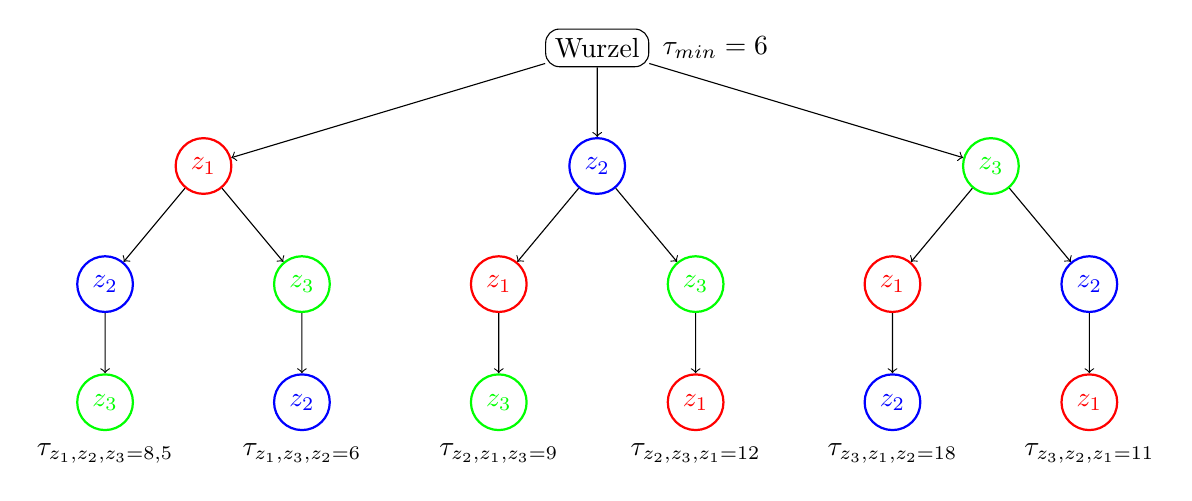
\begin{tikzpicture}[->,level/.style={sibling distance = 5cm/#1,
  level distance = 1.5cm}]
\node[rectangle, draw, rounded corners=5] (root) {Wurzel}
	child { node[red]{$z_1$}
		child { node[blue]{$z_2$}
			child { node[green](1){$z_3$} }
		}
		child { node[green]{$z_3$}
			child { node[blue](2){$z_2$} }
		}
	}
	child { node[blue]{$z_2$}
		child { node[red]{$z_1$}
			child { node[green](3){$z_3$} }
		}
		child { node[green]{$z_3$}
			child { node[red](4){$z_1$} }
		}
	}
	child { node[green]{$z_3$}
		child { node[red]{$z_1$}
			child { node[blue](5){$z_2$} }
		}
		child { node[blue]{$z_2$}
			child { node[red](6){$z_1$} }
		}
	};	
\node[above of=root, yshift=-1cm, xshift=1.5cm] {$\tau_{min} = 6$};
\node[below of=1, yshift=0.35cm] {$\tau_{z_1,z_2,z_3 = 8,5}$};
\node[below of=2, yshift=0.35cm] {$\tau_{z_1,z_3,z_2 = 6}$};
\node[below of=3, yshift=0.35cm] {$\tau_{z_2,z_1,z_3 = 9}$};
\node[below of=4, yshift=0.35cm] {$\tau_{z_2,z_3,z_1 = 12}$};
\node[below of=5, yshift=0.35cm] {$\tau_{z_3,z_1,z_2 = 18}$};
\node[below of=6, yshift=0.35cm] {$\tau_{z_3,z_2,z_1 = 11}$};
\end{tikzpicture}
\end{figure}

\begin{figure}[htbp]
\centering
\caption{Mit der Brute-Force-Optimierung wird direkt hinter $z_3$ abgeschnitten, da an diesem Knoten bereits der Zeitpunkt $\tau_{min}$ überschritten wird.}
\label{fig:BF2}
\begin{tikzpicture}[->,level/.style={sibling distance = 5cm/#1,
  level distance = 1.5cm}]
\node[rectangle, draw, rounded corners=5] (root) {Wurzel}
	child { node[red]{$z_1$}
		child { node[blue]{$z_2$}
			child { node[green]{$z_3$} }
		}
		child { node[green]{$z_3$}
			child { node[blue]{$z_2$} }
		}
	}
	child { node[blue]{$z_2$}
		child { node[red]{$z_1$}
			child { node[green]{$z_3$} }
		}
		child { node[green]{$z_3$}
			child { node[red]{$z_1$} }
		}
	}
	child { node[green](z3){$z_3$}
		child { node[gray]{$z_1$}
			child { node[gray]{$z_2$} }
		}
		child { node[gray]{$z_2$}
			child { node[gray]{$z_1$} }
		}
	};	
\node[above of=root, yshift=-1cm, xshift=1.5cm] {$\tau_{min} = 6$};
\node[below of=1, yshift=0.35cm] {$\tau_{z_1,z_2,z_3 = 8,5}$};
\node[below of=2, yshift=0.35cm] {$\tau_{z_1,z_3,z_2 = 6}$};
\node[below of=3, yshift=0.35cm] {$\tau_{z_2,z_1,z_3 = 9}$};
\node[below of=4, yshift=0.35cm] {$\tau_{z_2,z_3,z_1 = 12}$};
\node[right of=z3, xshift=0.2cm] {$\tau_{z_3} = 6.5$};
\node[red, thick, cross out, below, xshift=4.3cm, yshift=-2.1cm, rotate=50] { };
\node[red, thick, cross out, below, xshift=5.7cm, yshift=-2.1cm, rotate=-50] { };
\end{tikzpicture}
\end{figure}

\chapter{Experimente}


%\chapter{Conclusion}
\chapter{Zusammenfassung und Ausblick}
\textcolor{red}{TODO}



\begin{bibtex-entries}
@article{helvig,
  title={The moving-target traveling salesman problem},
  author={Helvig, Christopher S and Robins, Gabriel and Zelikovsky, Alex},
  journal={Journal of Algorithms},
  volume={49},
  number={1},
  pages={153--174},
  year={2003},
  publisher={Elsevier}
}

@article{moraes,
  title={Experimental Analysis of Heuristic Solutions for the Moving Target Traveling Salesman Problem Applied to a Moving Targets Monitoring System},
  author={de Moraes, Rodrigo S and de Freitas, Edison P},
  journal={Expert Systems with Applications},
  year={2019},
  publisher={Elsevier}
}

@inproceedings{hammar,
  title={Approximation results for kinetic variants of TSP},
  author={Hammar, Mikael and Nilsson, Bengt J},
  booktitle={International Colloquium on Automata, Languages, and Programming},
  pages={392--401},
  year={1999},
  organization={Springer}
}

@incollection{brandstadt1994kurzeste,
  title={K{\"u}rzeste Wege},
  author={Brandst{\"a}dt, Andreas},
  booktitle={Graphen und Algorithmen},
  pages={106--123},
  year={1994},
  publisher={Springer}
}
\end{bibtex-entries}



% If you need to have an appendix (I advise against it), insert it
% here using, first, \appendix and then \chapter and then,
% possibly, \section. 
%
% \appendix
%
% \chapter{Technical Appendix}
%
% \section{Experimental Parameters} % possibly
%
% Again, I advise against using an appendix.


\end{document}

%\begin{lemma|proof}
